%%%%%%%%%%%%%%%%%%%%%%%%%%%%%%%%%%%%%%%%%%%%%%%%%%%%%%%%%%%%%%%%%%%%%%%%%%%%%%%%
\section{Krótka geneza Internetu}
%%%%%%%%%%%%%%%%%%%%%%%%%%%%%%%%%%%%%%%%%%%%%%%%%%%%%%%%%%%%%%%%%%%%%%%%%%%%%%%%

Za początek pracy, nad powszechnie znanymi dziś technologiami internetowymi, uznaje się lata 60-te XX wieku. Wówczas, wybitni przedstawiciele środowisk informatycznych, rozpoczęli pracę nad nowym sposobem przesyłu danych ,zwanym komutacją pakietów.

Wedle udokumentowanej w literaturze historii Internetu \cite{Leiner.history-of-internet}, istniały aż trzy niezależne od siebie źródła pracy nad ideą komutacji pakietów: 

\begin{itemize}
    \item Działalność akademicka naukowców z MIT (Massachusetts Institute of Technology) w Stanach Zjednoczonych. Opracowana przez nich teoria, została wykorzystana do stworzenia pierwszego na świecie prototypu rozległej sieci komputerowej (WAN) przy pomocy sieci telefonicznej.
    \item Badania naukowe NPL (National Physical Laboratory) w Anglii, w których po raz pierwszy użyto terminu "pakiet" wobec jednostek danych.
    \item Projekt niezawodnego systemu komunikacji dla armii Stanów Zjednoczonych, stworzony przez działaczy organizacji badawczej RAND (Research And Development), z udziałem Paula Barana \cite{Baran.komutacja-pakietow}.
\end{itemize}

Wyniki pracy każdego z zespołów, przełożyły się na projekt rewolucyjnej sieci ARPANET, tworzonej pod patronatem amerykańskiej organizacji DARPA (Defense Advanced Research Projects Agency). Z początku łączyła ona jedynie Uniwersytet Kalifornijski i ośrodek naukowy SRI (Stanford Research Institute). W roku 1968 przeprowadzona została pierwsza pomyślna transmisja host-to-host między tymi węzłami. 

ARPANET, w kolejnych latach, został rozbudowany o wiele nowych węzłów, osadzonych głównie w akademickich placówkach badawczych, pozostając wciąż tajemnicą dla opinii publicznej. Zdecydowanym krokiem naprzód, było ostateczne dopracowanie protokołu NCP (Network Control Program), ściśle określającego przebieg przesyłu pakietów za pośrednictwem urządzeń IMP (Interface Message Processor). Same urządzenia IMP stanowiły pierwszą generację urządzeń, zwanych bramami sieciowymi, stanowiących mediator między komunikującymi się przez ARPANET komputerami (hostami), podłączonymi do dwóch różnych sieci lokalnych (LAN). Umożliwiło to stworzenie, pierwszych znaczących aplikacji do przesyłu plików i komunikatów, między hostami tworzonej sieci WAN.

ARPANET, po raz pierwszy został zaprezentowany publicznie w 1972 roku na konferencji ICCC (International Computer Communication Conference), spotykając się z entuzjastycznym odbiorem. W tym samym roku, przedsiębiorstwo BBN Technologies, utworzyło oprogramowanie umożliwiające skorzystanie z pierwszej w historii sieci email, za pośrednictwem sieci ARPANET, dokonując przełomu w metodach komunikacji międzyludzkiej.

Ewolucja sieci ARPANET, w znany dzisiaj powszechnie Internet, była wynikiem wielu zmian i ogromnego nakładu pracy wizjonerów, którzy kształtowali nowy porządek w dziedzinie sieci komputerowych. Szczegółowe opisanie każdego z etapów tego procesu, znacznie wykracza poza zakres tworzonej pracy. Poniżej przedstawiono wyłącznie najważniejsze nurty kształtujące dzisiejszy Internet:

\begin{itemize}
    \item Pierwotni architekci sieci ARPANET, zdecydowali się na obranie nowej strategii, polegającej na tworzeniu sieci, zgodnie z zasadą otwartej architektury. Regułą stało się opracowywanie ogólnodostępnych standardów i specyfikacji, umożliwiających twórcom oprogramowania i sprzętu komputerowego, tworzenie kompatybilnych ze sobą rozwiązań, mogących w pełni wykorzystywać możliwości sieci Internet. Wspomniane dokumenty od 1969 roku, są publikowane i komentowane w ramach zbioru Request for Comments (RFC) \cite{RFC.index}. Dużą rolę w rozpowszechnianiu i rozwoju tych standardów, odgrywa organizacja Internet Engineering Task Force (IETF).
    \item Protokół NPC wraz z urządzeniami IMP ze względu na swoje ograniczenia, zostały zastąpione przez nowsze odpowiedniki - protokół TCP/IP oraz współpracujące z nimi nowe generacje bram sieciowych. Z początku protokół kontroli transmisji (TCP) oraz protokół internetowy (IP) stanowiły jedną nierozłączną całość, by następnie zostać rozdzielone na dwie niezależne od siebie specyfikacje.
    \item We wrześniu 1981 roku, opublikowana została specyfikacja RFC 791, stanowiąca opis czwartej wersji protokołu IP \cite{RFC.791.IP}, która do dziś jest dominującym standardem identyfikowania komputerów w internecie.
    \item Ostateczne zaprzestanie eksploatacji protokołu NPC na rzecz stosu TCP/IP zostało zaplanowane na 1 stycznia 1983 roku i przebiegło zaskakująco pomyślnie. Dzięki tej ważnej zmianie, w drugiej połowie lat 80-tych XX wieku, na rynku zaczęły pojawiać się pierwsze oferty komercyjnych dostawców usług internetowych (ISP).
\end{itemize}

Mimo prężnego rozwoju technologii internetowych, u podstaw ich działania wciąż leży idea komutacji pakietów. Zgodnie z jej metodologią, przesyłany strumień danych musi zostać podzielony na mniejsze jednostki zwane pakietami. Każdy pakiet zawiera porcje danych oraz swój nagłówek wykorzystywany do jego identyfikacji. Tak przygotowane pakiety przesyłane są przez węzły sieci, podlegając niezależnemu od innych pakietów trasowaniu (tj. wyboru kolejnych węzłów, przez które zostaną przesłane do odbiorcy).

%%%%%%%%%%%%%%%%%%%%%%%%%%%%%%%%%%%%%%%%%%%%%%%%%%%%%%%%%%%%%%%%%%%%%%%%%%%%%%%%
\section{Epoka World-Wide Web}
%%%%%%%%%%%%%%%%%%%%%%%%%%%%%%%%%%%%%%%%%%%%%%%%%%%%%%%%%%%%%%%%%%%%%%%%%%%%%%%%

W końcówce lat 80-tych XX wieku, Internet, na przekór swoim ogromnym możliwościom, wciąż pozostawał mało wygodnym narzędziem, zarówno dla twórców oprogramowania jak i użytkowników przeszukujących sieć w celu uzyskania informacji. W następstwie tego, w 1989 roku, Tim Berners-Lee, informatyk pochodzenia brytyjskiego, rozpoczął pracę nad projektem WorldWideWeb (WWW lub W3) \cite{Berners-Lee.world-wide-web}. Projekt zakładał opracowanie prostszej i przystępniejszej metody wykorzystania sieci internetowej.

Założeniem nowego sposobu eksploracji zasobów, udostępnionych za pośrednictwem Internetu, było przenoszenie się po zawartości plików hipertekstowych przy pomocy umieszczonych w nich odnośników (linków). Koncepcja WWW korzystała z architektury klient-serwer, w której zadaniem klienta było przetwarzanie kompleksowej warstwy prezentacji, a zadaniem serwerów wydajne przeszukiwanie i manipulacja danymi.

By osiągnąć zamierzony efekt, opracowano nowy protokół HTTP (Hypertext Transfer Protocol), służący komunikacji klienta z serwerem. Zapewniał on nowe funkcjonalności, takie jak uzyskiwanie plików tekstowych po ich nazwie, czy przeszukiwanie spisu dokumentów po frazie podanej przez użytkownika, przy użyciu pojedynczych połączeń TCP/IP. Protokół ten do dziś, stanowi główny sposób wykorzystywania usług internetowych przez ich użytkowników, wraz z jego wersją HTTPS dodającą możliwość szyfrowania wysyłanych żądań. 

Dużą rolę w działaniu sieci WWW, odgrywają unikatowe identyfikatory zasobów URI. Specyfikacja ta umożliwia identyfikacje zasobów udostępnionych w ramach serwerów HTTP przy pomocy ciągu znaków. Identyfikatory najczęściej kojarzone są ze ścieżkami do pojedynczych plików, znanych z systemów operacyjnych. Pierwotnie URI zostały opracowane w dokumencie RFC 2396 przez Bernersa-Lee oraz jego współpracowników. Jednakże podobnie jak inne internetowe standardy, podlegają rewizji w nowszych dokumentach z tej serii \cite{rfc.2396.URI}.

Kluczowym narzędziem w technologiach WWW, jest oprogramowanie znane jako przeglądarki internetowe. Głównych zadaniem tych programów jest wysyłanie i odbiór żądań HTTP oraz odpowiedzi na te żądania. Dodatkowo, pełnią one rolę interpretera odbieranych plików hipertekstowych, wyświetlając wygenerowany na ich podstawie tekst, odnośniki, multimedia oraz elementy interfejsu użytkownika.

We wrześniu 1990 roku, Tim Berners-Lee stworzył pierwszy w historii serwer HTTP o nazwie httpd oraz narzędzie klienckie WorldWideWeb. Było ono, jednocześnie przeglądarką internetową, jak i edytorem plików hipertekstowych. Stworzony prototyp został pozytywnie przyjęty przez użytkowników, a WWW zaczęło zyskiwać coraz większą rzeszę zwolenników.

W 1994 roku, Berners-Lee założył organizację World Wide Web Consortium (W3C), zrzeszającą zwolenników sieci WWW. Jej główną misją jest promowanie i rozwój technologii W3, poprzez tworzenie i ulepszanie rządzących nią protokołów oraz specyfikacji. Umożliwia to produktywne tworzenie i aktualizowanie przeglądarek internetowych przez niezależnych twórców oraz łatwy rozwój aplikacji internetowych. Dzięki temu, sieć WWW jest obecnie najpopularniejszym na świecie sposobem eksploatacji Internetu, a standardy z nią związane, potocznie nazywane są "technologiami webowymi" \cite{W3C.about}.

%%%%%%%%%%%%%%%%%%%%%%%%%%%%%%%%%%%%%%%%%%%%%%%%%%%%%%%%%%%%%%%%%%%%%%%%%%%%%%%%
\section{Hipertekstowy język znaczników HTML}
%%%%%%%%%%%%%%%%%%%%%%%%%%%%%%%%%%%%%%%%%%%%%%%%%%%%%%%%%%%%%%%%%%%%%%%%%%%%%%%%

Podstawą działania stron internetowych WWW są dokumenty hipertekstowe. Na potrzeby przetestowania swojej nowej koncepcji, twórca WorldWideWeb sformułował pierwszą specyfikację hipertekstowego języka znaczników (HTML) w 1990 roku. Jednakże, nie traktowano jej jako oficjalnego standardu. Dopiero w 1993 roku, członkowie organizacji IETF, rozpoczęli tworzenie wersji roboczej oficjalnej specyfikacji, ostatecznie dokończonej z ramienia W3C w 1995 roku. Standardowi, stworzonemu dla użytkowników Internetu, nadano nazwę HTML 2.0 \cite{RFC.1866.HTML-2}. 

W końcówce lat 90-tych XX wieku, standard HTML otrzymał jeszcze kilka rewizji, rozbudowujących go o nowe funkcjonalności, kończąc na wersji HTML 4.01 w 1999 roku. W maju 2000 roku, międzynarodowa organizacja normalizacyjna (ISO) utworzyła standard ISO/IEC 15445:2000, hipertekstowego języka znaczników bazujący bezpośrednio na HTML 4.01 \cite{ISO.HTML}.

Przez ponad dekadę, specyfikacja HTML nie podlegała większym zmianom, aż do 2014 roku. Wtedy to, opublikowana została wersja HTML 5.0 kompleksowo przekształcająca możliwości dokumentów hipertekstowych i wprowadzająca wiele nowych znaczników. Decydujący wpływ na rozwój piątej wersji języka HTML, miała założona specjalnie w tym celu grupa Web Hypertext Application Technology Working Group (WHATWG). 

Podczas gdy organizacja W3C zajęta była rozwojem nowego standardu XHTML, grupa WHATWG tworzyła rozwiązanie kompatybilne ze starszymi wersjami języka HTML. Niektóre nowości ze standardu XHTML 1 stały się również elementami HTML5.  Grupa WHATWG jest obecnie częścią W3C odpowiedzialną za aktualizowanie standardu w jego podwersjach. Spekuluje się, że HTML5 zostanie rekomendowaną wersją, jeszcze przez co najmniej kilka następnych lat, będąc rozwijanym jako żywy standard, otrzymujący częste aktualizacje i uzupełnienia \cite{html.whatwg}.

Dokumenty napisane w hipertekstowym języku znaczników, są plikami tekstowymi zawierającymi znaczniki występujące w nawiasach ostrych np. <html>, <div> czy <img>. Najczęściej znaczniki te, występują w parach - pierwszy ze znaczników nazywany jest znacznikiem początkowym (otwierającym), a drugi znacznikiem końcowym (zamknięcia). Dodatkowo, znacznik końcowy odróżnia znak "/" przed jego nazwą np. otwierający <html> i zamykający </html>. W języku HTML wyróżniamy również znaczniki pojedyncze jak np. <img>, reprezentujący obraz cyfrowy występujący na stronie. 

Jako dodatkowy opis elementu reprezentowanego przez znacznik, wykorzystuje się tzw. atrybuty. Atrybuty to wartości opisane przez łańcuch znaków, przypisane do odpowiednich nazw wewnątrz nawiasów <> znacznika rozpoczynającego. Mogą one występować w dowolnej kolejności, jednakże zawsze po nazwie opisywanego znacznika. Należy również zaznaczyć fakt, że w rozpoznawaniu nazw znaczników i ich atrybutów, nie występuje rozróżnienie na małe i duże litery tj. <HTML> jest równoznacznym znacznikiem z <html>.

\begin{lstlisting}[language=HTML, caption=Przykładowy dokument HTML5, label=lst:html.example]
    <!DOCTYPE html>
    <html lang="pl">
    	<head>
            <meta http-equiv="content-type" content="text/html" charset="utf-8">
            <meta http-equiv="content-language" content="pl">
            <title>Tytuł tej strony</title>
    	</head>
    	<body>
            <header>
                <img src="https://via.placeholder.com/200x150?text=LOGO_STRONY">
                <h1>Tytuł strony</h1>
            </header>
            <nav>
                <ul>
                    <li><a href="home.html">Strona główna</a></li>
                    <li><a href="forum.html">Forum</a></li>
                    <li><a href="about.html">O nas</a></li>
                    <li><a href="contact.html">Kontakt</a></li>
                <ul>
            </nav>
            
            <section>
                <h2>Sekcje dzielą główną treść strony na części</h2>
                <article>
                    <h4>Dodatkowy podział sekcji na artykuły</h4>
                    <p>Każda sekcja może zostać dodatkowo podzielona na artykuły
                    takie jak ten.</p>
                </article>
                <article>
                    <h4>Warto korzystać z nowych znaczników HTML5</h4>
                    <p>Mimo, że nie jest to wymagane, korzystne jest zastosowanie 
                    nowej konwencji w swoich projektach.</p>
                </article>
            </section>
            
            <aside>
                <img src="https://via.placeholder.com/120x240?text=Reklama">
            </aside>
            
            <footer>
                <img src="https://via.placeholder.com/100x75?text=LOGO_W_STOPCE">
                <p>Strona testowa 2021</p>
            </footer>
        </body>
    </html>
\end{lstlisting}

Na listingu \ref{lst:html.example} przedstawiony został przykładowy plik HTML. Zgodnie z zaleceniami W3C, dokumenty publikowane w internecie rozpoczynają się od deklaracji ich typu, aby przeglądarka internetowa otrzymała informacje jaki plik przetwarza. Pliki HTML5 rozpoczynają się od linii <!DOCTYPE html>. Następnie otwierany jest znacznik <html> wyznaczający granice dokumentu hipertekstowego.

Wewnątrz znacznika <html> zagnieżdżone zostały dwa kolejne. Znacznik <head> pełni funkcję nagłówka strony poświęconemu jej metadanym. Metadane, wykorzystywane są, aby zapewnić przeglądarce internetowej oraz oprogramowaniu przeszukującemu Internet, dodatkowe informacje przyczyniające się do poprawnego zinterpretowania treści dokumentu. Przykładowo zostały przedstawione trzy znaczniki metadanych:

\begin{itemize}
    \item Pierwszy znacznik <meta>, zawiera atrybuty określające sposób kodowania pliku. Dzięki temu znaki specjalne zostaną wyświetlone w przeglądarce w prawidłowy sposób.
    \item Atrybuty drugiego znacznika <meta> określają język w jakim napisany jest dokument. Informacja ta może zostać wykorzystana do automatycznego tłumaczenia strony przy pomocy dodatkowego oprogramowania.
    \item Ostatni znacznik <title> definiuje nazwę strony, która zostanie wyświetlona w opisie karty w przeglądarce internetowej.
\end{itemize}

Kolejnym znacznikiem zagnieżdżonym w <html> jest <body>. W jego wnętrzu, zdefiniowane jest całe ciało strony, czyli wszystkie elementy, widoczne w obrębie okna przeglądarki. Przestrzegając reguł narzuconych przez specyfikacje języka, twórcy dokumentu są w stanie modelować wyświetlaną strukturę elementów, w dowolny sposób. Standard HTML5 wprowadził jednak zbiór znaczników semantycznych, ułatwiających tworzenie struktury, przejrzystej zarówno dla użytkowników przeglądających Internet, jak i dla innych programistów czytających kod źródłowy strony.

\begin{figure}[!htbp] 
    \centering
    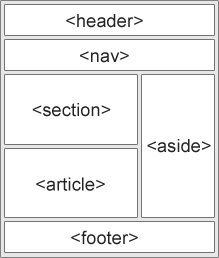
\includegraphics{img/chapter3/html.semantic-elements.png}
    \caption{Przykładowy diagram struktury elementów semantycznych z oficjalnej strony W3C}
    \label{fig:html.semantic-elements}
\end{figure}

Znaczniki semantyczne to takie, których nazwa wskazuje na przetrzymywaną w nich zawartość. Pierwszym elementem w proponowanej na rys. \ref{fig:html.semantic-elements} strukturze jest <header>. Zgodnie z nazwą, jest to nagłówek strony, w którym powinny zostać umieszczone elementy takie jak logo, tytuł lub motto. Następny to <nav> reprezentujący elementy nawigacyjne, takie jak wysuwany boczny panel lub horyzontalną belkę, zawierające odnośniki do stron tworzących najważniejsze sekcje portalu internetowego. Linki zagnieżdżone w elemencie <nav> rozpoznawane są przez nowoczesne wyszukiwarki internetowe, jako podelementy strony głównej portalu, ułatwiając szybki dostęp do wybranych treści.

Następne dwa popularne znaczniki to <section> oraz <article>. Najczęściej wykorzystuje się je do podziału głównej treści danej strony na pomniejsze części. Innym znacznikiem semantycznym o podobnym przeznaczeniu jest <main> wykorzystywany do okalania całej treści głównej, tak jak robi to <header> z nagłówkiem. Element <aside> użyty został do okalania zawartości znajdującej się na bok od treści głównej. W przykładowym listingu \ref{lst:html.example} jest to wertykalny baner reklamowy. 

Strukturę strony kończy stopka, zawarta w elemencie <footer>. Stopka zwyczajowo używana jest do wyświetlenia informacji o twórcach strony oraz latach w których rozwijano portal. Czasami zawiera alternatywne linki nawigacyjne oraz gwarantuje szybki dostęp do informacji kontaktowych \cite{Mazur.html5-css3}.

\begin{figure}[!htbp] 
    \centering
    
\includegraphics[width=\textwidth]{img/chapter3/html.example.rendered.png}
    \caption{Przykładowa strona wyświetlona przez przeglądarkę na podstawie dokumentu z listingu \ref{lst:html.example}}
    \label{fig:html.example.rendered}
\end{figure}

Na rys. \ref{fig:html.example.rendered} przedstawiona została strona internetowa wyświetlona przez przeglądarkę na podstawie listingu \ref{lst:html.example}. Mimo nie najgorszej przejrzystości wyświetlanej treści, strona nie wygląda szczególnie ciekawie czy oryginalnie. Język HTML został wzbogacony o znaczniki i atrybuty, umożliwiające w ograniczonym stopniu modyfikację wyglądu wyświetlanych elementów. Nie są one jednak dobrym narzędziem do osiągnięcia tego celu. Aby efektywnie zapobiec monotonii stron internetowych, opracowane zostały kaskadowe arkusze stylów, opisane w następnej sekcji.

%%%%%%%%%%%%%%%%%%%%%%%%%%%%%%%%%%%%%%%%%%%%%%%%%%%%%%%%%%%%%%%%%%%%%%%%%%%%%%%%
\section{Kaskadowe arkusze stylów CSS}
%%%%%%%%%%%%%%%%%%%%%%%%%%%%%%%%%%%%%%%%%%%%%%%%%%%%%%%%%%%%%%%%%%%%%%%%%%%%%%%%

W 1994 roku, działacze W3C pracujący nad językiem HTML, rozważyli propozycję stworzenia kaskadowych arkuszy stylów (CSS), których zadaniem byłoby uproszczenie procesu stylizacji stron internetowych. Jako efekty tych prac, wyróżnia się rekomendację CSS1 (1996) oraz uzupełniającą ją CSS2 (1998). Od 2004 do 2011 roku, rozwijana była specyfikacja CSS2.1. Jednakże, w 2011 roku, podjęta została decyzja o podziale specyfikacji kaskadowych arkuszy stylów na pomniejsze, rozwijane niezależnie od siebie moduły.

W tym samym roku, udostępnione zostały moduły selektorów, kolorów i przestrzeni nazw poziomu trzeciego, bazujące na wersjach CSS2.1, a rekomendowaną specyfikacją stał się CSS3. Większość modułów CSS3, osiągnęła już trzeci poziom swojego rozwoju, ale nowe zaczynają rozwój od poziomu pierwszego, jak na przykład popularny moduł Flexbox, opublikowany w 2017 roku. Istnieją już moduły na poziomie 4, co zapowiada możliwą zmianę rekomendowanego standardu na CSS4 w najbliższej dekadzie. 

Arkusz CSS, stworzony jest z reguł, opisujących style elementów dokumentu hipertekstowego. Każda reguła składa się z selektora i deklaracji. Selektory są wskaźnikami na elementy, które powinny zostać ustylizowane przez daną regułę. Najczęściej selektorami są znaczniki elementów z dokumentu HTML. Deklaracja zawiera natomiast właściwości oraz przypisane im wartości.

Kaskadowość arkuszy CSS, polega na hierarchii ważności poszczególnych stylów, opisanych przy ich pomocy. Tworząc je, należy pamiętać o wyższym priorytecie bardziej szczegółowych selektorów, np. selektor wskazujący na elementy listy ma pierwszeństwo nad wskazującym na listę jako całość. Ponadto, arkusze stylów wystąpić mogą w jednej z trzech opisanych poniżej form:

\begin{itemize}
    \item Style lokalne - sformułowane jako atrybuty konkretnego elementu HTML. Każdy element HTML może posiadać atrybut "style" wewnątrz którego, znajdą się stylizujące go deklaracje. Niektóre elementy posiadają unikalne atrybuty tworzące deklaracje stylizujące np. element <img> posiada atrybuty "width" i "height" pozwalające zadeklarować szerokość i wysokość wyświetlanego obrazka.
    \item Wewnętrzny arkusz stylów występujący w nagłówku pliku hipertekstowego. Arkusz wewnętrzny zagnieżdżony jest w specjalnym elemencie <style>.
    \item Zewnętrzny plik CSS - dołączany do pliku hipertekstowego w jego nagłówku. Dodatkową korzyścią z zastosowania tej metody jest możliwość uwzględnienia  arkusza stylów z wielu plików jednocześnie.
\end{itemize}

W celu zaprezentowania każdej z trzech metod, na listingach  \ref{lst:css.local-style-example} oraz \ref{lst:css.head-style-example} przedstawione zostały zmodyfikowane fragmenty pliku HTML z listingu \ref{lst:html.example}.

\begin{lstlisting}[language=HTML, caption=Przykład stylu lokalnego CSS w dokumencie HTML, label=lst:css.local-style-example]
<nav>
    <ul>
      <li><a href="index.html" style="color: #f6f7eb;"><div>Strona główna</div></a></li>
      <li><a href="forum.html"><div>Forum</div></a></li>
      <li><a href="about.html"><div>O nas</div></a></li>
      <li><a href="contact.html"><div>Kontakt</div></a></li>
    </ul>
</nav>
\end{lstlisting}

Najwyższy priorytet posiadają selektory określone jako styl lokalny dla wybranego elementu HTML. Na listingu \ref{lst:css.local-style-example} jako przykład, zastosowano styl określający kolor czcionki, na biały,  dla odnośnika wskazującego na obecnie przeglądaną stronę (plik index.html).

\begin{lstlisting}[language=HTML, caption=Przykład stylów CSS zastosowanych przy pomocy nagłówka dokumentu HTML, label=lst:css.head-style-example]
<head>
  <meta http-equiv="content-type" content="text/html" charset="utf-8">
  <meta http-equiv="content-language" content="pl">
  <title>Tytuł tej strony</title>
  <link rel="stylesheet" href="node_modules/normalize.css/normalize.css" type="text/css">
  <style type="text/css">
    body {
      margin: 0;
      padding: 0;
      color: #f6f7eb;
      background-color: #5c414d;
      font-family: 'Akaya Kanadaka', sans-serif;
    }
  </style>
  <link rel="stylesheet" href="css/small.css" type="text/css">
  <link rel="stylesheet" href="css/medium.css" type="text/css">
  <link rel="stylesheet" href="css/large.css" type="text/css">
</head>
\end{lstlisting}

Listing \ref{lst:css.head-style-example} rozbudowuje nagłówek strony o element <style> w obrębie którego, można dowolnie definiować selektory CSS. Dołączanie zewnętrznych arkuszy CSS, realizowane jest przy pomocy elementów <link> z atrybutami definiującymi typ i ścieżkę do pliku.

\begin{lstlisting}[language=HTML, caption=Fragment pliku small.css załączonego w nagłówku dokumentu HTML, label=lst:css.example.small]
nav>ul>li>a {
  color: #cf8e80;
  text-decoration: none;
  font-size: larger;
}

nav>ul>li>a>div {
  padding: 0.4em 2em;
  text-align: center;
}

nav>ul>li>a>div:hover {
  background-color: #f6f7eb42;
}

main {
  padding: 1.5em;
  background-color: #f6f7eb10;
  display: grid;
  grid: auto-flow min-content / 1fr;
  grid-gap: 2em;
  justify-items: center;
}

section {
  display: grid;
  grid: auto-flow min-content / 1fr;
  grid-gap: 0.6em
}

article>h4, footer>p {
  color: #cf8e80;
}

#commercial-vertical {
  display: none;
}

#commercial-horizontal {
  display: block;
}
\end{lstlisting}

\begin{figure}[!htbp] 
    \centering
    
\includegraphics[width=\textwidth]{img/chapter3/css.example.small.png}
    \caption{Przykładowa strona z listingu \ref{lst:html.example} po zastosowaniu kaskadowych arkuszy stylów}
    \label{fig:css.example.small}
\end{figure}


Priorytet deklaracji stylów określonych w załączonych plikach oraz elemencie <style> określa kolejność występowania w nagłówku. Przy każdym wystąpieniu tego samego selektora, dodaje się deklaracje niezdefiniowane wcześniej oraz nadpisuje się wartości tych, które zostały już użyte.

Obecnie jednym z najważniejszych zastosowań kaskadowych arkuszy stylów, jest dostosowywanie sposobu wyświetlania treści na stronie do rozdzielczości ekranu.  Jest to możliwe dzięki nowym zapytaniom typu media poziomu 3. Cecha ta jest nazywana potocznie responsywnością aplikacji.
Dla HTML4 oraz CSS2 w specyfikacji istniało już słowo kluczowe "media"  pozwalające dostosować wyświetlaną treść do określonego typu dokumentu tj. strona internetowa czy dokument do wydruku. Poziom 3, umożliwił natomiast dostosowywanie deklaracji CSS do parametrów wyświetlania dokumentu, takich jak szerokość oraz wysokość, aspekt czy orientacja strony wyświetlanej na urządzeniu \cite{css.media-queries}.

\begin{lstlisting}[language=CSS, caption=Plik medium.css załączony w nagłówku dokumentu HTML, label=lst:css.example.medium]
@media only screen and (min-width: 720px) {
  header {
    grid: min-content max-content / min-content min-content; 
    align-items: center;
  }
    
  main {
    grid: auto-flow min-content / 1fr min-content;
    align-items: center;
  }

  #commercial-vertical {
    display: block;
  }

  #commercial-horizontal {
    display: none;
  }
}
\end{lstlisting}

\begin{lstlisting}[language=CSS, caption=Plik large.css załączony w nagłówku dokumentu HTML, label=lst:css.example.large]
@media only screen and (min-width: 1024px) {
  nav>ul {
    grid: auto-flow min-content / 1fr 1fr 1fr 1fr;
  }
}
\end{lstlisting}

Przykładowo na listingach \ref{lst:css.example.medium} oraz \ref{lst:css.example.large} przedstawiono zapytanie media w plikach medium.css i large.css. Podmieniają one deklaracje dotyczące sposobu wyświetlania elementów na stronie, na ekranach, których szerokość wynosi kolejno przynajmniej 720 i 1024 pikseli.

\begin{figure}[!htbp] 
    \centering
    
\includegraphics[width=\textwidth]{img/chapter3/css.example.medium.png}
    \caption{Przykładowa strona internetowa dla ekranów o szerokości większej niż 1024 pikseli}
    \label{fig:css.example.medium}
\end{figure}

Rzeczywiste zmiany sposobu wyświetlania strony względem rys. \ref{fig:css.example.small} można zaobserwować na rys. \ref{fig:css.example.medium}. Dzięki zastosowaniu kwerend media w ten sposób, zmiany zostały wprowadzone przyrostowo. Linki w nagłówku strony ułożono w sposób bardziej horyzontalny, a obrazek reprezentujący reklamę przesunięto na boczny panel strony.

%%%%%%%%%%%%%%%%%%%%%%%%%%%%%%%%%%%%%%%%%%%%%%%%%%%%%%%%%%%%%%%%%%%%%%%%%%%%%%%%
\section{JavaScript i model obiektowy dokumentu}
%%%%%%%%%%%%%%%%%%%%%%%%%%%%%%%%%%%%%%%%%%%%%%%%%%%%%%%%%%%%%%%%%%%%%%%%%%%%%%%%

Za pomocą opisanych w poprzednich sekcjach standardów HTML oraz CSS jesteśmy w stanie tworzyć dobrze przemyślane, atrakcyjne wizualnie i responsywne interfejsy użytkownika. Jednakże szybko okazuje się, że strony internetowe bazujące jedynie na tych dwóch technologiach, stanowią bardzo sztywne, praktycznie statyczne treści.

Dzięki funkcjonalnościom selektorów i deklaracji CSS poziomu trzeciego, jesteśmy w stanie definiować proste animacje do odegrania na elementach HTML, czy nawet odpowiedzi na interakcje, takie jak przykrycie kursorem powierzchni elementu. Wciąż jednak okazuje się, że te rozwiązania obarczone są dużymi ograniczeniami i wymagają dużej wprawy przy tworzeniu złożonych elementów interaktywnych.

Na potrzebę łatwiejszej implementacji elementów interaktywnych, jako pierwsi spróbowali odpowiedzieć pracownicy firmy Netscape Communications. Po ogromnym sukcesie ich przeglądarki Netscape Navigator w latach 90-tych XX wieku, początkowo zakładali oni zastosowanie jednego z popularnych wówczas języków programowania takich jak Java, Perl czy Python. Ostatecznie podjęto decyzję o zaimplementowaniu zupełnie nowego języka skryptowego na potrzeby programu Netscape Navigator 2.

W 1995 roku, Brendan Eich, rozpoczął pracę nad technologią nazwaną początkowo Mocha. Podczas dystrybucji wersji beta nowej przeglądarki, nazwę języka zmieniono początkowo na LiveScript , by następnie przemianować ją na znany do dziś JavaScript (JS).

W wyniku pozytywnego przyjęcia wersji JS 1.0, zarząd firmy Microsoft zadecydował o stworzeniu własnej, konkurencyjnej implementacji języka o nazwie JScript. Został on dołączony do przeglądarki Internet Explorer 3 w okresie zbliżonym do daty wydania programu Netscape Navigator 3, wyposażonego w nowe funkcjonalności JS 1.1. Niestety technologie te nie były ze sobą w pełni kompatybilne, zmuszając twórców aplikacji do tworzenia kilku wersji swoich produktów, w celu dostarczenia ich do większej rzeszy użytkowników.

Z uwagi na powyższe, w 1997 roku, firma Netscape zadecydowała o utworzeniu powszechnie dostępnego standardu ECMA-262 z pomocą instytucji ECMA International. ECMA jako organizacja powołana w celu ustanawiania oraz dystrybucji nowych norm w dziedzinie komunikacji i przetwarzania informacji, do dziś stanowi rzetelne źródło informacji o standardzie JavaScript.

Dzięki pracy fundacji Mozilla (pochodnej od przedsiębiorstwa Netscape) oraz instytucji ECMA International, twórcy przeglądarek internetowych są w stanie implementować rozwiązania kompatybilne z przeglądarkami różnych dostawców. Podobnie jest w przypadku standardów rozwijanych przez W3C oraz dystrybuowanych jako dokumenty RFC \cite{js.history}.

Aby wykorzystać pełen potencjał języka JS, potrzebne są odpowiednie interfejsy programistyczne (Web API), definiujące zbiór obiektów i funkcji, dające dostęp do zaawansowanych funkcjonalności przeglądarek:

\begin{itemize}
    \item Możliwość manipulacji elementami dokumentu HTML oraz ich atrybutami,  zapewnia interfejs programistyczny modelu obiektowego dokumentu (DOM API) \cite{js.dom}.
    \item W aplikacjach wykorzystujących mapy lub dostosowujące język wyświetlania strony automatycznie, przydatne bywa API odpowiadające za funkcjonalności związane z geolokacją użytkownika (Geolocation API). 
    \item Dostępne powszechnie interfejsy płótna (Canvas API) oraz WebGL API, umożliwiające tworzenie kolejno dwuwymiarowych oraz trójwymiarowych obrazów animowanych.
    \item Interfejsy umożliwiające zaawansowaną obsługę multimediów audiowizualnych w postaci buforowanych strumieni takich jak HTMLMediaElement czy WebRTC.
\end{itemize}

Są to jedynie najpopularniejsze przykłady interfejsów, dostępnych domyślnie w większości popularnych przeglądarek. Nie należy zapominać o istnieniu wielu interfejsów dostępnych jako oprogramowanie stron trzecich. Ich kod można załączyć na własną rękę w projekcie własnej strony internetowej, udostępniając ich funkcjonalności użytkownikowi końcowemu \cite{js.docs}.

\begin{lstlisting}[language=JavaScript, caption=Treść przykładowego skryptu JavaScript w pliku script.js, label=lst:js_example_script]
const logo = document.querySelector('header>img');
const title = document.querySelector('header>h1')

logo.addEventListener('click', onLogoClick);

function onLogoClick() {
    const name = prompt('Podaj nowy tytuł strony:');
    title.textContent = name;
}

\end{lstlisting}

Jako przykładowy skrypt JS na listingu \ref{lst:js_example_script} przedstawiono wykorzystanie DOM do pobrania obiektowej reprezentacji elementów obrazka i tytułu z nagłówka strony. Następnie zdefiniowano funkcję wywoływaną w odpowiedzi na zdarzenie kliknięcia kursorem na ten obrazek. 

\begin{lstlisting}[language=HTML, caption=Wykorzystanie skryptów JavaScript w pliku HTML, label=lst:js_in_html]
<script src="js/script.js" defer></script>
<script>
  // tu również można umieścić treść skryptu
</script>
\end{lstlisting}

Chcąc korzystać ze skryptów w dokumencie HTML należy użyć elementu <script>. Istnieje możliwość zastosowania go na dwa sposoby ukazane na listingu \ref{lst:js_in_html}:

\begin{itemize}
    \item Załączenie zewnętrznego pliku *.js - wykorzystując atrybut src, możemy w czytelny sposób załączyć wiele skryptów logicznie podzielonych na moduły w osobnych plikach.
    \item Wewnętrzny skrypt - w zawartości elementu <script> można zawrzeć w pełni funkcjonalny kod JavaScript, mogący odwoływać się do selektorów i identyfikatorów obecnego dokumentu.
\end{itemize}

Wynik wywołania zdarzenia obsłużonego na listingu \ref{lst:js_example_script} przedstawiono na rys. \ref{fig:js.example.prompt}. Funkcja onLogoClick() wykorzystuje API wbudowane w przeglądarkę internetową, aby ukazać monit, pozwalający na wprowadzenie nowej zawartości elementu dla tytułu strony.

\begin{figure}[!htbp] 
    \centering
    
\includegraphics[width=\textwidth]{img/chapter3/js.example.prompt.png}
    \caption{Monit wyświetlony na skutek zdarzenia kliknięcia kursorem na logo przykładowej strony HTML}
    \label{fig:js.example.prompt}
\end{figure}

Po potwierdzeniu wprowadzenia nowej nazwy, podmieniona zostaje wartość pola textContent w obiekcie reprezentującym element HTML. Zmiany wprowadzone przy pomocy obiektów interfejsu DOM są widoczne w strukturze dokumentu na rys. \ref{fig:js.example.after_click}.

\begin{figure}[!htbp] 
    \centering
    
\includegraphics[width=\textwidth]{img/chapter3/js.example.after_click.png}
    \caption{Nagłówek przykładowej strony HTML po wprowadzeniu nowej zawartości tytułu w monicie na rys. \ref{fig:js.example.prompt}}
    \label{fig:js.example.after_click}
\end{figure}

%%%%%%%%%%%%%%%%%%%%%%%%%%%%%%%%%%%%%%%%%%%%%%%%%%%%%%%%%%%%%%%%%%%%%%%%%%%%%%%%
\section{Nowy standard WebAssembly}
%%%%%%%%%%%%%%%%%%%%%%%%%%%%%%%%%%%%%%%%%%%%%%%%%%%%%%%%%%%%%%%%%%%%%%%%%%%%%%%%

W dzisiejszych czasach, Internet wypełniony jest interaktywną zawartością, w której najważniejszą rolę odgrywa język programowania JavaScript (JS). To z jego pomocą, twórcy aplikacji klienckich są w stanie dynamicznie manipulować elementami HTML, czy deklaracjami CSS na oczach użytkownika np. przy pomocy identyfikatorów HTML. Ponadto, umożliwia on wysyłanie żądań HTTP oraz obsługę odbioru ich odpowiedzi, za pośrednictwem dedykowanych w tym celu, interfejsów programistycznych, tworząc istotną warstwę logiki w tych aplikacjach.

Jednakże w 2015 roku, pojawił się nowy standard nazwany WebAssembly (WASM), który w 2019 roku został włączony w poczet technologii rekomendowanych przez W3C. Miał on początkowo odpowiadać na potrzebę wykonywania kodu po stronie użytkownika, z wydajnością bliską natywnej. JS pozostaje wysokopoziomowym językiem skryptowym, z pamięcią zarządzaną automatycznie oraz kodem optymalizowanym dynamicznie w czasie kompilacji w locie. WASM przypomina raczej niskopoziomowy kod asemblera, odrzucającego m.in. wtórne optymalizacje kodu oraz czytelny dla człowieka format, na rzecz bardzo szybkiej egzekucji w silniku przeglądarki \cite{wasm.concepts}.

WASM jest językiem statycznie typowanym i definiuje jedynie cztery podstawowe typy danych - liczby całkowite w wariantach 32-bit i 64-bit oraz liczby zmiennoprzecinkowe, również w wariantach 32-bit i 64-bit. Jego działanie opiera się na czterech podstawowych pojęciach opisanych poniżej:

\begin{itemize}
    \item Moduł - kompaktowy plik binarny definiujący bezstanowy kod wykonywalny. Umożliwia to współdzielenie pliku przez kilka osobnych instancji na raz. Ze względu na format binarny można przesyłać go w postaci strumienia bajtów i przeprowadzić jego interpretacje na bieżąco.
    \item Pamięć - bufor o zmiennym rozmiarze, stanowiący tablice bajtów nadpisywanych i czytanych przez niskopoziomowy system pamięci WebAssembly. Każdy z bajtów posiada własny indeks, który może zostać potraktowany jako adres w pamięci w określonych przypadkach.
    \item Tablica - bufor o zmiennym rozmiarze, służący do przechowywania referencji, które nie powinny być przechowywane jako bajty w pamięci WASM, np. referencje do funkcji.
    \item Instancja - moduł wraz z przypisaną do niego pamięcią i tablicą oraz wszystkimi zaimportowanymi wartościami. Instancja w odróżnieniu od modułu jest więc obarczona stanem.
\end{itemize}

WebAssembly nie został wprowadzony by zastąpić język JavaScript, a raczej stać się jego współpracownikiem w realizacji określonych zadań. Dzięki interfejsom programistycznym (definiujących m.in. powyższe 4 pojęcia) wprowadzonym do standardów, możliwa jest komunikacja dwukierunkowa między obiema technologiami w przeglądarce.

Przykładowo, pozwala to na szybkie wykonanie obliczeń przy pomocy zaimportowanego modułu WASM w aplikacji klienckiej, stworzonej głównie w języku JS. Analogicznie, możliwa jest nawet manipulacja strukturami DOM strony internetowej wewnątrz modułu WASM, wykorzystując JS jako mediator. Na chwilę obecną DOM i WebAssembly nie mogą komunikować się w żaden sposób bezpośrednio, jednakże rozważa się wprowadzenie tej możliwości w kolejnych wersjach standardu.

Zaletą binarnego WASM, jest możliwość zastosowania formatu, jako cel kompilacji dla innych technologii. W ten sposób, języki takie jak C++, Rust czy C\# mogą zostać wykorzystane do tworzenia funkcjonalnych modułów dla internetowych aplikacji klienckich. Przykładowymi zastosowaniami takiego rozwiązania, są szybkie obliczenia, na potrzeby renderowania grafiki przy pomocy interfejsu WebGL, przetwarzania plików audiowizualnych, obliczeń kryptograficznych czy kompresji.

Niektóre platformy programistyczne wychodzą jednak o krok dalej, umożliwiając tworzenie w pełni funkcjonalnych aplikacji klienckich, przy pomocy języków innych niż JS. Jest to możliwe, dzięki wprowadzeniu warstwy inter-operatywności, przy pomocy pośredniej technologii WASM. Z takiego właśnie rozwiązania, korzystano podczas tworzenia projektu, opisywanego dalej w niniejszej pracy.

%%%%%%%%%%%%%%%%%%%%%%%%%%%%%%%%%%%%%%%%%%%%%%%%%%%%%%%%%%%%%%%%%%%%%%%%%%%%%%%%
\section{Najważniejsze cechy protokołu HTTP}
%%%%%%%%%%%%%%%%%%%%%%%%%%%%%%%%%%%%%%%%%%%%%%%%%%%%%%%%%%%%%%%%%%%%%%%%%%%%%%%%

W poprzednich sekcjach, omówione zostały najważniejsze technologie webowe, pozwalające użytkownikom na interakcje ze stronami internetowymi, zgodnie z wizją Tima Bernesa-Lee. Jednakże, ich prawidłowe funkcjonowanie jest możliwe, dzięki zastosowaniu protokołu HTTP \cite{http.docs}, dostarczającemu ich zasoby do klienta.

Aby przybliżyć naturę tego protokołu, w kontekście opisywanej pracy, poniżej wypunktowano kilka jego najważniejszych cech ze stosownymi objaśnieniami:

\begin{itemize}
    \item HTTP jest protokołem warstwy aplikacji - oznacza to, że stanowi część najbardziej abstrakcyjnej warstwy Internetu. W odróżnieniu od protokołów TCP (warstwa transportu) oraz IP (warstwa internetowa) jego głównym zadaniem jest reprezentacja przesyłanych danych w sposób łatwo interpretowany przez interfejsy aplikacji klienckich i serwerowych.
    \item Stanowi on przykład implementacji modelu klient-serwer, w którym, zadaniem klienta jest wysłanie zapytania do serwera i interpretacja odpowiedzi jakiej udzielił.
    \item Bezstanowość oznacza, że między odpowiedziami na kolejne żądania, serwer nie przetrzymuje informacji o ich stanie. Substytutem do tego, są tzw. ciasteczka, stanowiące mechanizm stanu sesji, związany bezpośrednio z protokołem HTTP. Więcej informacji o nich zamieszczono w następnej sekcji pracy.
\end{itemize}

Żądanie HTTP składa się z trzech wymaganych elementów, ale może zawierać dodatkowo, kilka opcjonalnych nagłówków oraz ciało (body) reprezentujące przesyłane dane. Jego treść zawsze rozpoczyna tzw. metoda.

\begin{itemize}
    \item Metoda GET odpowiada za pobieranie zasobów z serwera. W odpowiedzi można spodziewać się zwrotu treści dokumentu HTML, pliku graficznego lub nawet pojedynczego łańcucha znaków.
    \item Metoda POST służy głównie do tworzenia encji w bazie danych lub np. obsługi procesu uwierzytelniania użytkownika w systemie. W odróżnieniu od żądań GET przesyła w swoim ciele dane, które następnie przetworzy aplikacja serwerowa.
    \item Kolejnymi często stosowanymi metodami są PUT i PATCH, służące do aktualizacji danych encji w bazie danych. Podobnie jak żądania POST zwykle zawierają w swoim ciele dane, jednak odróżnia je sposób wprowadzania zmian. PUT symbolizuje ponowne wstawienie całego rekordu w bazie ze zaktualizowanymi wartościami, podczas gdy PATCH skupia się na podmianie wybranych wartości w jego komórkach.
    \item Ostatnią podstawową metodą jest DELETE, służąca do usuwaniu zasobów po stronie serwera, wykorzystując np. klucz główny rekordu w bazie danych.
\end{itemize}

Metody pełnią głównie rolę semantyczną, pozwalając programistom na łatwiejsze zrozumienie, jaką rolę powinny odgrywać tworzone akcje. Ich rolą nie jest ograniczenie możliwości wykonywanych operacji po stronie serwera.  Nie narzucają również ograniczeń na dołączone w żądaniu nagłówki i zawartość danych w ciele żądania.

\begin{lstlisting}[caption=Przykładowe rządanie HTTP, label=lst:http.example_request]
GET /?q=HTTP&t=h_ HTTP/2
Host: duckduckgo.com
User-Agent: Mozilla/5.0 (Windows NT 10.0; rv:91.0) Gecko/20100101 Firefox/91.0
Accept: text/html,application/xhtml+xml,application/xml;q=0.9,image/avif,image/webp,*/*;q=0.8
Accept-Language: en-US,en;q=0.5
Accept-Encoding: gzip, deflate, br
DNT: 1
Connection: keep-alive
Upgrade-Insecure-Requests: 1
Sec-Fetch-Dest: document
Sec-Fetch-Mode: navigate
Sec-Fetch-Site: same-origin
Sec-Fetch-User: ?1
TE: trailers
\end{lstlisting}

Pozostałymi dwoma niezbędnymi elementami żądania, jest ścieżka określająca adres punktu końcowego na który, powinno zostać wysłane żądanie oraz kod wykorzystywanej wersji protokołu. Umieszczenie kolejno metody, adresu oraz kodu wersji, oddzielonych spacjami w pierwszym wierszu przesyłanych danych, tworzy prawidłowe i kompletne żądanie HTTP. 

W celu wykorzystania pełni potencjału żądań warto jest zastosować opcjonalne nagłówki. Są one parami wartości przypisanych do zdefiniowanych przez standard kluczy, oddzielonych od siebie znakiem nowej linii. Przykładowo, wykorzystanie nagłówka "Host" pozwala nam zdefiniować prefiks do ścieżki punktu końcowego i znacznie skrócić pierwszy wiersz żądania.

Fragment żądania nazywany ciałem, od jego nagłówków odgranicza jedna pusta linia. Najczęściej dane sformatowane są jako notacja obiektowa JavaScript (JSON) przez wzgląd na jej czytelność dla ludzi i maszyn. Może on także przedstawiać dane w formacie binarnym lub dowolną treść tekstową.

Odpowiedzi HTTP od żądań, odróżnia zawartość ich pierwszej linii. Zamiast metody, pierwszym jej elementem, jest kod wersji stosowanego protokołu, drugim kod statusu wykonanego żądania, a ostatnim wiadomość opisująca ten status. W przypadku dodatkowych nagłówków oraz ciała odpowiedzi, sytuacja jest identyczna jak dla żądań.

\begin{lstlisting}[caption=Odpowiedź HTTP na przykładowe żądanie z listingu \ref{lst:http.example_request}, label=lst:http.example_response]
HTTP/2 200 OK
server: nginx
date: Sat, 29 Jan 2022 20:03:24 GMT
content-type: text/html; charset=UTF-8
vary: Accept-Encoding
...
x-duckduckgo-locale: en_US
content-encoding: br
X-Firefox-Spdy: h2

<!DOCTYPE html>...
\end{lstlisting}

Wśród kodów statusu odpowiedzi HTTP, wyróżniamy pięć głównych podgrup, obsługujących pokrewne ze sobą sytuacje. Każdy z kodów statusu jest trzycyfrową liczbą całkowitą. Pierwsza z cyfr określa przynależność do jednej z podgrup, a pozostałe dwie służą sprecyzowaniu z jakim przypadkiem klient ma do czynienia. Statusy x00 najczęściej reprezentują sytuacje, w których trudno jest skonkretyzować naturę otrzymanego wyniku.

\begin{itemize}
    \item Kody 1xx odpowiadają za sytuacje, w których klient może kontynuować wykonywaną operację lecz powinien otrzymać pewne metadane dotyczące swojego żądania. Na przykład, stosując w żądaniu nagłówek "Expected: 100-continue" można wymusić na serwerze przesłanie informacji zwrotnej ze statusem "100 Continue", świadczącej o prawidłowym użyciu nagłówków w żądaniu HTTP.
    \item Statusy powodzenia 2xx określają, że żądanie zostało wykonane pomyślnie. Przykładowo "204 Created" informuje o pomyślnym utworzeniu nowego zasobu po stronie serwera.
    \item Przekierowania 3xx obsługują wszystkie te sytuacje, w których zaszła potrzeba przekierowania żądania użytkownika na inny adres. Ciekawym przykładem jest status "304 Not Modified" implikujący możliwość skorzystania z utworzonej wcześniej w pamięci podręcznej kopii zasobu, ze względu na brak zmian w jego treści od ostatniego uzyskanego dostępu.
    \item Niepowodzenia żądań 4xx - jednoznacznie wskazują na to, że mimo uzyskania połączenia z serwerem i obsłużenia żądania, operacja zakończyła się niepowodzeniem. Jednym z najpopularniejszych kodów statusu w internecie, jest bez wątpienia "404 Not Found" informujący o tym, że punkt końcowy do którego chcemy uzyskać dostęp nie został odnaleziony. 
    \item Wewnętrzne błędy serwera 5xx stanowią zdecydowanie najbardziej zatrważające ze statusów odpowiedzi HTTP. W ich przypadku, serwer nie działa poprawnie, dlatego nie jest w stanie obsłużyć przesyłanego żądania. 
\end{itemize}

Dzięki swej prostocie, protokół HTTP jest w stanie zapewnić deweloperom bardzo przejrzysty i dobrze udokumentowany sposób komunikacji klienta z serwerem. Począwszy od sformułowania standardu, liczba jego zastosowań wciąż rośnie i prawdopodobnie pozostanie on kluczowym rozwiązaniem w dziedzinie informatyki przez kilka najbliższych dekad.

%%%%%%%%%%%%%%%%%%%%%%%%%%%%%%%%%%%%%%%%%%%%%%%%%%%%%%%%%%%%%%%%%%%%%%%%%%%%%%%%
\section{Ciasteczka HTTP, pamięć sesji i pamięć lokalna}
%%%%%%%%%%%%%%%%%%%%%%%%%%%%%%%%%%%%%%%%%%%%%%%%%%%%%%%%%%%%%%%%%%%%%%%%%%%%%%%%

W poprzedniej sekcji, przedstawione zostały podstawowe założenia protokołu HTTP, który w rękach wprawnego inżyniera oprogramowania, stanowi bardzo uniwersalne narzędzie. Jednakże, jego bezstanowość zainicjowała potrzebę wykorzystania dodatkowego mechanizmu, odpowiedzialnego za przechowywanie informacji o stanie klienta bądź serwera.

Na potrzebę tą, jako pierwsze odpowiedzieć miały ciasteczka HTTP, nazywane w skrócie "ciasteczkami", opisane w dokumencie RFC 6265 \cite{cookies.rfc6265}. Stan sesji klienta, bądź serwera, jest przechowywany przy ich pomocy w przeglądarce użytkownika, jako pliki składujące klucz oraz przypisaną do niego wartość \cite{cookies.docs}.

\begin{lstlisting}[caption=Przykładowa odpowiedź HTTP wykorzystująca nagłówek Set-Cookie, label=lst:cookies.setCookies]
HTTP/2 200 OK
Content-Type: text/html
Set-Cookie: ciasteczko_1=wartość_1
Set-Cookie: ciasteczko_2=wartość_2
...

[Zawartość strony]
\end{lstlisting}

Do tworzenia plików ciasteczek służy nagłówek Set-Cookie, dołączany w odpowiedzi HTTP przez serwer. Na listingu \ref{lst:cookies.setCookies} zaprezentowano bardzo prosty przykład jego wykorzystania tworzący dwa pliki ciasteczek, nieobarczonych żadnymi dodatkowymi ograniczeniami, nazwane kolejno ciasteczko\_1 oraz ciasteczko\_2.

\begin{lstlisting}[caption=Przykładowe żądanie HTTP wykorzystujące nagłówek Cookies, label=lst:cookies.cookies_header]
GET /search HTTP/2
Cookies: ciasteczko_1=wartość_1; ciasteczko_2=wartość_2
\end{lstlisting}

W wyniku składowania plików ciasteczek w pamięci przeglądarki, zostają one automatycznie dołączone do każdego kolejnego żądania wysyłanego na serwer, który je utworzył. Przeglądarka robi to przy pomocy nagłówka Cookies w sposób przedstawiony na listingu \ref{lst:cookies.cookies_header}.

Mechanizm plików ciasteczek posiada kilka dodatkowych funkcjonalności, umożliwiających wykorzystanie ich w bardziej wyspecjalizowany sposób. Przy pomocy tzw. atrybutów ciasteczka jesteśmy w stanie wyznaczyć okres ich ważności, zabezpieczyć ich zawartość przed niewłaściwym użyciem, a także uściślić sposób ich automatycznego załączania.

\begin{lstlisting}[caption=Przykładowe użycie atrybutu terminu ważności ciasteczka HTTP, label=lst:cookies.expires]
Set-Cookie: ciasteczko_1=wartość_1; Expires=Tue, 08 Feb 2022 10:00:00 GMT;
Set-Cookie: ciasteczko_2=wartość_2; Max-Age: 20;
\end{lstlisting}

Ciasteczko, dla którego nie ustawiono terminu ważności, jest ważne do końca trwania obecnej sesji przeglądarki. W przypadku skorzystania z atrybutu Expires, serwer jest w stanie ustalić moment, w którym plik utraci swą ważność. Nowszy atrybut Max-Age ułatwia pracę z tym mechanizmem, pozwalając na określenie, po ilu sekundach od momentu przesłania ciasteczka przez serwer, ulega ono przedawnieniu. Po upływie tego terminu, ciasteczko domyślnie zostaje usunięte z pamięci przeglądarki.

\begin{lstlisting}[caption=Przykładowe użycie atrybutów dostępu ciasteczka HTTP, label=lst:cookies.secure]
Set-Cookie: ciasteczko_1=wartość_1; Secure; HttpOnly
Set-Cookie: ciasteczko_2=wartość_2; HttpOnly
\end{lstlisting}

Kolejnymi atrybutami ciasteczek są flagi Secure oraz HttpOnly, użyte przykładowo na listingu \ref{lst:cookies.secure}, odpowiadające za zakres dostępu. W przypadku pierwszego z nich, blokuje się dostęp do wartości ciasteczek, żądaniom stosującym niezaszyfrowany wariant protokołu HTTP. Drugi, odpowiada za zablokowanie dostępu do ciasteczek językowi JavaScript, za pośrednictwem interfejsu DOM.

\begin{lstlisting}[caption=Przykładowe użycie atrybutów punktu docelowego ciasteczka HTTP, label=lst:cookies.domain]
Set-Cookie: ciasteczko_1=wartość_1; Domain=duckduckgo.com; Path=/search
Set-Cookie: ciasteczko_2=wartość_2; SameSite=Strict
\end{lstlisting}

Na listingu \ref{lst:cookies.domain} przedstawiono użycie trzech atrybutów, mających na celu uściślenie, do których żądań, należy dołączyć dane ciasteczko. W przypadku nie zastosowania atrybutu Domain, ciasteczka będą dołączane tylko do żądań prowadzących ściśle do hosta, który je utworzył. Atrybutu można użyć w celu całkowitej zmiany domeny lub adresu, jednakże powoduje on również rozszerzenie zakresu docelowych żądań na wszystkie poddomeny określonego adresu.

Atrybut Path, zawęża pulę żądań docelowych, do przypadków dotyczących konkretnych ścieżek. Przykładowo ciasteczko\_1 z listingu \ref{lst:cookies.domain} zostałoby dołączone jedynie do tych żądań, dla których domeną serwera byłoby "duckduckgo.com" lub jedna z jej poddomen np. "html.duckduckgo.com". Dodatkowo, lista ta podlega drugiemu przefiltrowaniu ścieżek do przypadków, w których zaczyna się ona od "/search", np. "/search", "/search/images" czy "/search/maps/pl".

Dodatkowy atrybut SameSite o podobnym zastosowaniu, odpowiada za przyjętą zasadę tolerancji wobec obcych domen. Od najnowszych zmian w standardzie ciasteczek, porównuje on wersje niezaszyfrowaną (http) oraz zaszyfrowaną (https) danej domeny, jako dwa osobne adresy. Jako atrybut typu wyliczeniowego, posiada trzy możliwe wartości:

\begin{itemize}
    \item Strict - wartość z pliku ciasteczka zostanie dołączona jedynie do żądań wychodzących ze strony, która początkowo je utworzyła.
    \item Lex - dodatkowo rozbudowuje powyższy tryb o przypadki przechodzenia z innej domeny na stronę, która utworzyła ciasteczko. Jest on trybem domyślnym.
    \item None - ciasteczka są wysyłane w żądaniach pochodzących zarówno ze strony stanowiącej ich źródło, jak i podczas przechodzenia na nią z obcej domeny, jednakże implikuje przymus użycia atrybutu Secure.
\end{itemize}


Pliki ciasteczek, dzięki swym atrybutom, umożliwiają automatyzację niektórych procesów związanych z przesyłaniem ich zawartości między klientem a serwerem. Przy odpowiednim zastosowaniu atrybutów, pozwalają magazynować stan sesji użytkownika przez ściśle określony czas i zadbać o jego bezpieczeństwo przed wieloma rodzajami ataków. 

Niestety, ciasteczka w dobie współczesnego internetu posiadają również wady. Pozwalają na przechowywanie maksymalnie 4096 bajtów danych, w ramach pojedynczego pliku. Zwykle, jest to pojemność wystarczająca do przechowywania metadanych użytkownika lub jego tokenu uwierzytelniającego (zalecany sposób przechowywania tych tokenów). Jednakże, twórcy przeglądarek internetowych postanowili odpowiedzieć na potrzebę większej rozszerzalności rozwiązań webowych.

\begin{figure}[!htbp] 
    \centering
    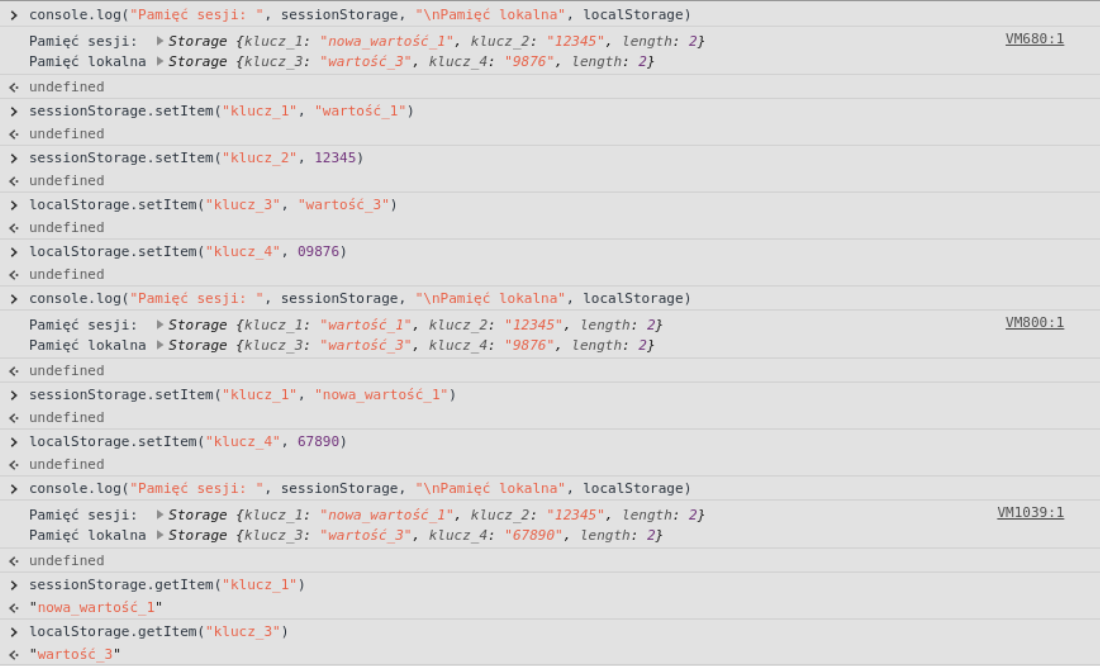
\includegraphics[width=\textwidth]{img/chapter3/storage.setting_values.png}
    \caption{Tworzenie, modyfikacja oraz dostęp do par klucz-wartość w pamięci sesji i pamięci lokalnej}
    \label{fig:storage.setting_values}
\end{figure}

Z tego powodu, zrodziła się idea interfejsu programistycznego pamięci webowej (Web Storage API), podzielonej na przestrzeń pamięci sesji oraz pamięci lokalnej \cite{web_storage.docs}. Opiera się ona na założeniu przypisywania danych do klucza. Jednakże, w odróżnieniu od plików ciasteczek, umożliwiła ona przechowywanie plików o pojemności od 5 do 10 megabajtów danych (w zależności od implementacji). Ponadto, dostęp do tej pamięci odbywa się w pełni za pośrednictwem skryptów JavaScript po stronie klienta. Na rys. \ref{fig:storage.setting_values} ukazano proces tworzenia, modyfikacji oraz dostępu do par klucz-wartość w obu rodzajach pamięci webowej przy pomocy jej interfejsu. Zarówno pamięć sesji, jak i pamięć lokalna, przypisane są do konkretnego źródła (domeny) w obrębie którego, można z nich skorzystać.

\begin{figure}[!htbp] 
    \centering
    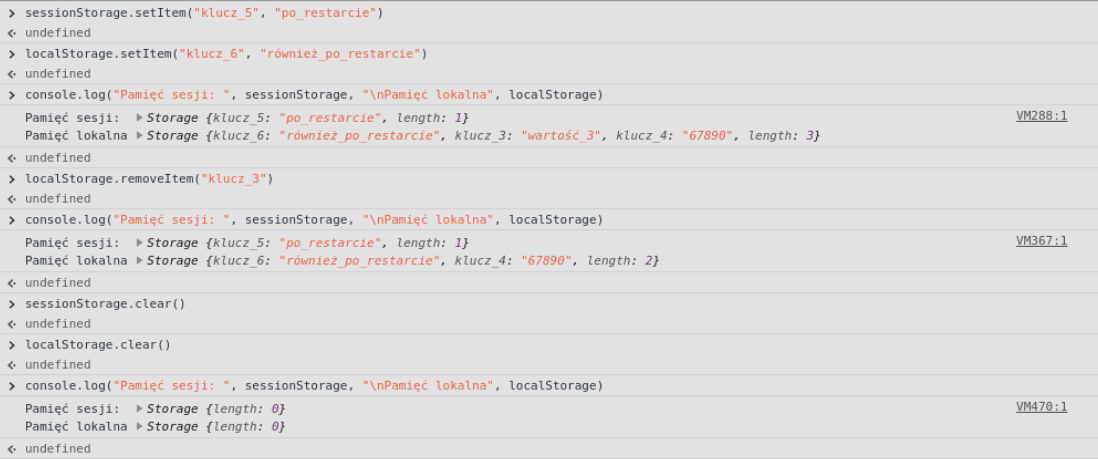
\includegraphics[width=\textwidth]{img/chapter3/storage.removing_values.png}
    \caption{Stan par klucz-wartość w pamięci sesji i pamięci lokalnej po ponownym uruchomieniu instancji przeglądarki oraz ręczne metody ich usuwania}
    \label{fig:storage.removing_values}
\end{figure}

Pamięć sesji, zgodnie ze swoją nazwą, służy do przechowywania danych, które zostaną automatycznie wykasowane z pamięci przeglądarki po zamknięciu instancji, w której zostały utworzone. Dane w pamięci lokalnej są w niej przetrzymywane, nawet po zamknięciu i ponownym uruchomieniu przeglądarki. Jedynym sposobem na usunięcie z niej zapisanych par kluczy i wartości, jest ręczne zastosowanie interfejsu programistycznego w skryptach strony lub wyczyszczenie ich z pamięci podręcznej, z poziomu ustawień samego programu. Procesy te zostały ukazane na rys. \ref{fig:storage.removing_values}, uchwyconym po ponownym uruchomieniu przeglądarki internetowej z rys. \ref{fig:storage.setting_values}.

Pliki ciasteczek i pamięć webowa, nie powinny być traktowane jako rywalizujące ze sobą rozwiązania tego samego problemu. Dzięki funkcjonalnościom, możliwym do zastosowania przy pomocy atrybutów ciasteczek oraz automatyzacji ich załączania, są one szczególnie pomocne w składowaniu danych stanu sesji istotnych dla aplikacji serwerowych systemu. Świetnie sprawdzą się w scenariuszach, w których liczy się bezpieczeństwo danych, łatwe przekazywanie metainformacji do wykorzystania przez inne domeny (np. logowanie B2C) oraz termin ważności tych informacji. 

Pamięć webowa, dzięki swej prostocie i ścisłemu związkowi ze skryptami wykonywanymi po stronie klienta, idealnie nadaje się do przechowywania danych, intensywnie wykorzystywanych przez aplikacje klienckie. To właśnie w nich, wykorzystany może zostać potencjał bardziej obszernych plików konfiguracyjnych, które może przechować dla nich nowszy mechanizm składowania stanu.

%%%%%%%%%%%%%%%%%%%%%%%%%%%%%%%%%%%%%%%%%%%%%%%%%%%%%%%%%%%%%%%%%%%%%%%%%%%%%%%%
\section{Tokeny JWT jako mechanizm autoryzacji}
%%%%%%%%%%%%%%%%%%%%%%%%%%%%%%%%%%%%%%%%%%%%%%%%%%%%%%%%%%%%%%%%%%%%%%%%%%%%%%%%

Jedną z ważniejszych oraz mniej oczywistych pozycji w stanie sesji klienta, stanowią dane autoryzacyjne klienta. W ostatnich latach, najpopularniejszym rozwiązaniem tego zagadnienia stały się tokeny JSON Web Tokens (JWT) \cite{jwt.rfc7519}. Swą popularność nad starszymi rozwiązaniami wykorzystującymi format XML \cite{jwt.auth0}, zawdzięczają kilku zaletom:

\begin{itemize}
    \item JWT oferują większe bezpieczeństwo, dzięki łatwości podpisywania tokenów w formacie JSON. Umożliwiają skorzystanie z puli algorytmów HMAC (bazującego na kluczu-sekrecie), RSA i ECDSA (klucz prywatny i publiczny). W porównaniu do podpisywania danych w formacie XML jest to o wiele prostszy proces.
    \item Obiektowość formatu JSON, jest powodem, nie tylko jego wysokiej czytelności dla ludzi, ale również, łatwego parsowania danych do obiektów w aplikacjach klienckich i serwerowych.
    \item Tokeny są bardzo kompaktowe, w porównaniu do  rozwiązań bazujących na formacie XML. Dają możliwość przesłania większej ilości danych w mniejszej ilości bajtów, w zakodowanej formie JWT.
\end{itemize}

Token JWT składa się z trzech części: nagłówka, ładunku i podpisu. Wszystkie trzy części przedstawiono w formie zakodowanej i zdekodowanej na rys. \ref{fig:jwt.parts}. Dwie pierwsze części, stanowią obiekty JS (znane z formatu JSON), ostatnia część jest wynikową operacji algorytmu podpisującego token.

\begin{figure}[!htbp] 
    \centering
    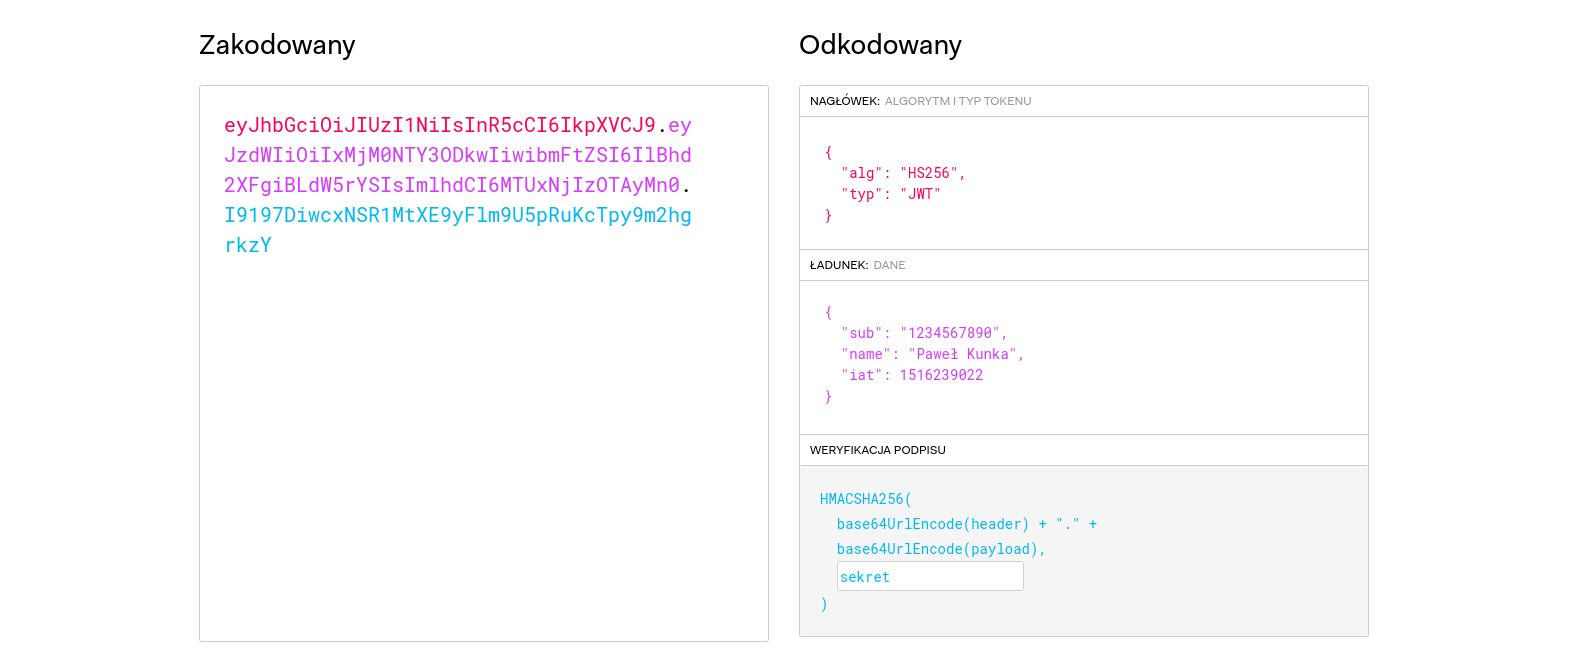
\includegraphics[width=\textwidth]{img/chapter3/jwt.parts.png}
    \caption{Analiza części składowych przykładowego tokenu JWT w formie zakodowanej i odkodowanej}
    \label{fig:jwt.parts}
\end{figure}

\begin{itemize}
    \item Nagłówek tokenu, przetrzymuje informacje o algorytmie używanym przy podpisywaniu i szyfrowaniu tokenu (pole alg) oraz typie tokenu (pole typ).
    \item Ładunek tokenu może, lecz nie musi, zawierać kilka pól tzw. twierdzeń, udostępniających dodatkowe informacje o encji, której poświęcony jest token np. dane użytkownika. Specyfikacja tokenów JWT, wyróżnia kilka twierdzeń zastrzeżonych, które służą konkretnym zastosowaniom. Ma to na celu zwiększenie kompatybilności rozwiązań. Przykładowo, użyte pola sub i iat służą kolejno do określenia identyfikatora encji, której został poświęcony token oraz czasu jego wyemitowania. Pole name jest twierdzeniem zdefiniowanym dodatkowo przez twórcę tokenu.
    \item Podpis jest ciągiem znaków, otrzymanym w wyniku zastosowania funkcji algorytmu podpisującego, określonego w nagłówku. Funkcja ta, przyjmuje za argumenty treść nagłówka i ładunku, oddzielonego kropką oraz tzw. sekret. Sekret jest ciągiem znaków, trzymanym w bezpiecznym miejscu, służącym do podpisywania i szyfrowania danych, po stronie jego właściciela. Podpis, pozwala potwierdzić autentyczność przesłanych informacji oraz czy wartości przedstawionych twierdzeń nie zostały zmodyfikowane.
\end{itemize}

Ze względu na bardzo mały rozmiar tokenów JWT, do ich przechowywania można zastosować zarówno pliki ciasteczek, jak i pamięć webową. Przez wzgląd na cechy ciasteczek, wymienione w poprzedniej sekcji, często stosuje się je w przypadku tokenów służących autoryzacji.

\begin{lstlisting}[caption=Użycie tokenu JWT jako mechanizm autoryzacji w żądaniu HTTP, label=lst:jwt.authorization]
Authorization: Bearer nagłówek_jwt.ładunek_jwt.podpis_jwt
\end{lstlisting}

Aby zastosować JWT w optymalny sposób, należy dołączyć do żądań, przesyłanych na zabezpieczone ścieżki serwera, nagłówek Authorization. Przykładowe użycie, zamieszczono na listingu \ref{lst:jwt.authorization}. Jego zawartość określa schemat wykorzystujący JWT jako element pośredni przenoszący dane (Bearer). 

%%%%%%%%%%%%%%%%%%%%%%%%%%%%%%%%%%%%%%%%%%%%%%%%%%%%%%%%%%%%%%%%%%%%%%%%%%%%%%%%
\section{Aplikacje serwerowe REST}
%%%%%%%%%%%%%%%%%%%%%%%%%%%%%%%%%%%%%%%%%%%%%%%%%%%%%%%%%%%%%%%%%%%%%%%%%%%%%%%%

W przypadku aplikacji serwerowych, zdecydowanie największą popularnością, cieszy się styl architektoniczny Reprezentacyjnego Transferu Stanu (REST lub aplikacja RESTowa). Jej koncepcję, zaproponował po raz pierwszy, doktor Roy Thomas Fielding w swojej pracy naukowej z roku 2000 \cite{restapi.genesis}. 

\begin{figure}[!htbp] 
    \centering
    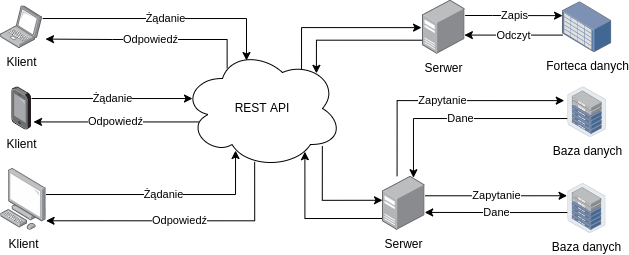
\includegraphics[width=\textwidth]{img/chapter3/rest.overview.png}
    \caption{Rola interfejsów programistycznych REST w systemach internetowych}
    \label{fig:rest.overview}
\end{figure}

Posiada on, kilka podstawowych założeń, nakładających na tworzone aplikacje ograniczenia, które ostatecznie przyczyniają się do tworzenia bardziej spójnego i rozszerzalnego rozwiązania. Poniżej przedstawiono podstawy architektury REST:

\begin{itemize}
    \item Ujednolicenie interfejsów - zasada mające swoje podłoże w paradygmacie ogólności inżynierii oprogramowania. Każdy interfejs, wskazujący na ten sam zasób, powinien wyglądać identycznie dla wszystkich źródeł swego pochodzenia np. dla każdego klienta. Interfejs REST powinien przekazywać ujednoliconą formę reprezentacji zasobu, na której powinien pracować klient. Interfejsy zasobów, powinny być jak najbardziej kompaktowe, jednocześnie zawierając w sobie wystarczającą porcję informacji opisujących przesyłaną wiadomość.
    \item Model klient-serwer - aplikacja kliencka powinna być świadoma istnienia jedynie tych identyfikatorów (ścieżek URI), które prowadzą do zasobów dostarczanych przez aplikacje serwerową. Jedyną ścieżką komunikacji między obydwoma programami powinien zostać protokół HTTP lub inny, jasno określony w dokumentacji interfejsu.
    \item Bezstanowość żądań - podobnie jak w przypadku protokołu HTTP, żądania REST są bezstanowe, wszystkie powinny w sobie zawierać wystarczającą ilość informacji, potrzebnych do ich przetworzenia i uzyskania odpowiedzi. Aplikacja serwerowa nie przetrzymuje informacji o statusie wcześniejszych żądań i uniemożliwia komunikację między nimi w ten sposób. Odpowiedzialność za przetrzymywanie stanu sesji może jednak zostać przerzucona na aplikację kliencką.
    \item Buforowalność - cecha zapewniająca w dłuższej perspektywie, skalowalność aplikacji serwerowej oraz lepszą wydajność aplikacji klienckiej. Aplikacja REST powinna udostępniać informacje o możliwości buforowania (przetrzymywania w pamięci podręcznej) otrzymanych wcześniej odpowiedzi po stronie klienta (lub serwera). Przykładowo, powinno być możliwe buforowanie obrazków, których znacznik czasu zapisu nie uległ zmianie w żądaniach poprzednich.
    \item Warstwowość - czasami to, co opisujemy jako aplikację RESTową, stanowi w rzeczywistości wiele pomniejszych, współpracujących ze sobą programów (np. mikro-serwisów). Cecha warstwowości opisuje abstrakcyjne założenie, zgodnie z którym, aplikacje klienckie, ani serwerowe nie zostają poinformowane, czy faktycznie komunikują się z końcowym wykonawcą danej operacji. Nie mają prawa żądać tej informacji, przyjmując interfejs programistyczny REST API jako obraz aplikacji serwerowej.
    \item Kod na żądanie - opcjonalna cecha REST, zakładająca dostarczenie części funkcjonalności systemu internetowego, w postaci kodu wykonywalnego po stronie użytkownika. Zgodnie z tą zasadą, taki kod powinien zostać uruchomiony jedynie za zgodą aplikacji klienckiej.
\end{itemize}

Opisane powyżej podstawowe założenia interfejsów programistycznych REST opierają się na pojęciu zasobów. Zasób jest pojęciem abstrakcyjnym, mogącym opisywać dowolną informację np. dokument HTML, obrazek, obiekt JS lub kolekcję takich obiektów.

Każdy zasób, posiada swój unikalny identyfikator, wykorzystywany w komunikacji między komponentami klienta i serwera. Stan zasobu nazywa się jego reprezentacją i dzieli na trzy główne składowe: dane zasobu, metadane zasobu, opisujące jego dane oraz łącza, które mogą okazać się pomocne przy zmianie jego stanu. Format danych reprezentacji, określa się jako typ medialny, który wykorzystuje się do określenia sposobu przetwarzania danego zasobu \cite{restapi.media_types.rfc6838}.

Przykładowo, dzięki typom medialnym zasobów, dokumenty HTML, arkusze CSS oraz obrazy, mogą zostać wyświetlone przez przeglądarkę, a dane przesłane w formacie JSON zmapowane na obiekty w aplikacji klienckiej lub serwerowej. Reprezentacja zasobów jest sama dla siebie opisem i nie zrzuca odpowiedzialności zinterpretowania swojej zawartości na klienta, ani serwer.

Istotnym elementem aplikacji RESTowych są również metody zasobów. Wykorzystuje się je w celu określenia, jaką operację należy zastosować na stanie zasobu. Bardzo często, metody zasobów traktuje się w sposób tożsamy z różnymi metodami żądań HTTP np. GET dla metody odczytującej zasób, POST dla metody tworzącej, PUT jako metoda aktualizacji, a DELETE jako usunięcie zasobu. Dzięki metodom zasobów można przeprowadzić kilka różnych operacji na tym samym zasobie, wykorzystując pojedynczy identyfikator (URI).

\begin{figure}[!htbp] 
    \centering
    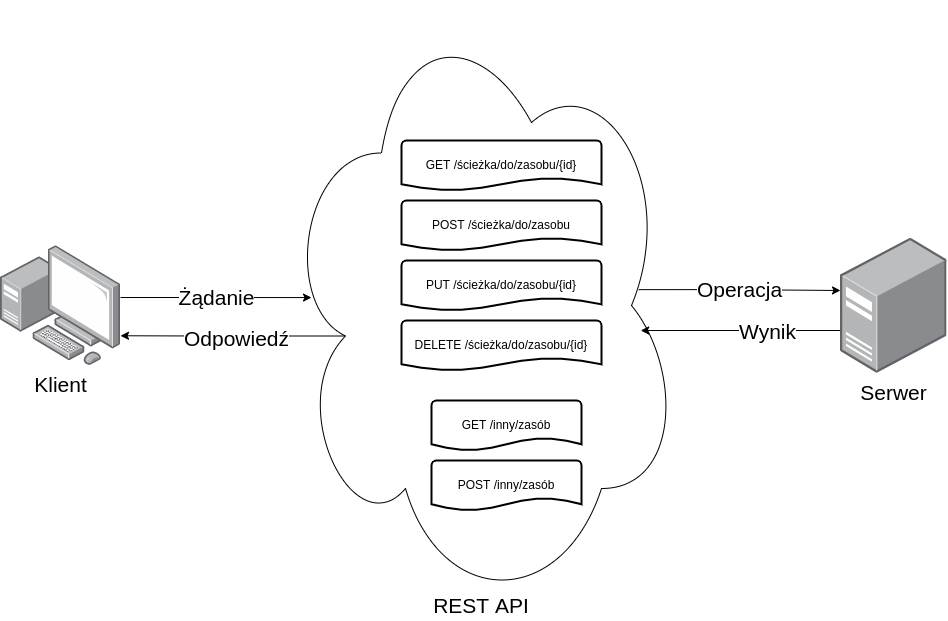
\includegraphics[width=\textwidth]{img/chapter3/rest.endpoints.png}
    \caption{Dostęp do zasobów poprzez punkty końcowe interfejsu REST}
    \label{fig:rest.endpoints}
\end{figure}

Podsumowując, interfejsy REST zakładają dostęp do funkcjonalności (operacji) i danych reprezentowanych przez jednostki zwane zasobami. Dostęp do danego zasobu odbywa się za pośrednictwem jego  ujednoliconego identyfikatora (URI) oraz odpowiedniej metody REST określającej rodzaj operacji do przeprowadzenia na zasobie.

Zasoby są wymieniane między klientem, a serwerem, w postaci swoich reprezentacji, które mogą definiować różne typy medialne np. tekst, HTML, XML, JSON czy PNG. Dzięki metadanym, możliwe jest buforowanie wybranych zasobów w celu zwiększenia wydajności systemu.

Reprezentacje zasobów przesyłane są między klientem a serwerem przy pomocy standaryzowanych interfejsów protokołu. W przypadku REST najczęściej jest to protokół HTTP, lecz architektura nie wymusza jego zastosowania. Ważne jest natomiast to, by serwer nie przetrzymywał stanu obsłużonych żądań ani sesji poszczególnych klientów.

%%%%%%%%%%%%%%%%%%%%%%%%%%%%%%%%%%%%%%%%%%%%%%%%%%%%%%%%%%%%%%%%%%%%%%%%%%%%%%%%
\section{Mechanizmy mapowania obiektowo-relacyjnego}
%%%%%%%%%%%%%%%%%%%%%%%%%%%%%%%%%%%%%%%%%%%%%%%%%%%%%%%%%%%%%%%%%%%%%%%%%%%%%%%%

Jednym z najważniejszych zadań aplikacji serwerowych jest często odczyt i zapis rekordów w bazach danych. Podstawową metodą dostępu do nich są, zdefiniowane przez dostawców silników bazodanowych, języki zapytań. Istnieje jednak alternatywny sposób pracy z nimi, zakładający wprowadzenie warstwy abstrakcji między bazą danych a aplikacją serwerową. 

Mapowanie obiektowo-relacyjne (ORM) to metoda, wywodząca się z domeny programowania obiektowego, zakładająca interakcję z bazami danych przy pomocy obiektów. Kluczową rolę pełni w niej klasa kontekstu bazy danych, stanowiąca interfejs programistyczny, pomiędzy kodem aplikacji serwerowej a bazą danych. Kontekst odpowiada za tworzenie zapytań, wykonujących operacje na rzeczywistych danych, interpretując zmiany wykonane na obiektach reprezentujących kolejno: tabele, rekordy i wartości poszczególnych komórek.

\begin{figure}[!htbp] 
    \centering
    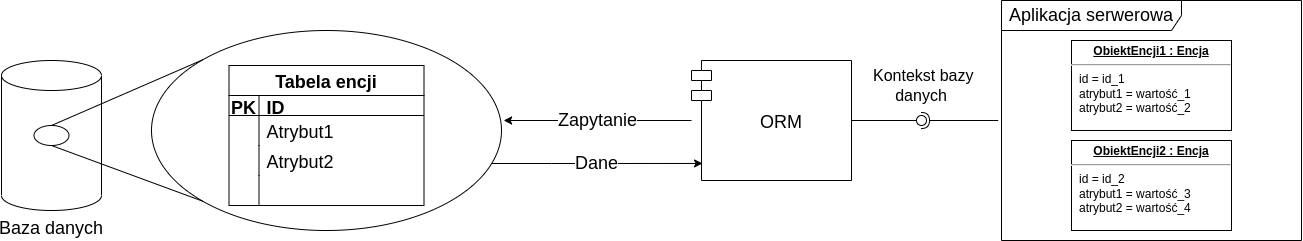
\includegraphics[width=\textwidth]{img/chapter3/orm.context.png}
    \caption{Zarys działania mapowania obiektowo-relacyjnego w aplikacjach serwerowych}
    \label{fig:orm.context}
\end{figure}

ORM najczęściej jest dołączany do projektu aplikacji jako osobna biblioteka programistyczna, zaimplementowana w języku programowania, kompatybilnym z rozwiązaniem. W praktyce, wyróżnia się trzy główne podejścia do rozpoczęcia pracy z tymi narzędziami:

\begin{itemize}
    \item Pierwszeństwo modelu bazy - metoda zakładająca wykorzystanie dedykowanego narzędzia do projektowania relacji w bazach danych, najczęściej przy pomocy diagramów opisanych w formacie pochodnym od standardu języka znaczników XML. Powstały w ten sposób model bazy danych, często może zostać wykorzystany przez ORM, do utworzenia relacji encji w bazie danych oraz wygenerowania klas encji w projekcie aplikacji serwerowej.
    \item Pierwszeństwo bazy danych - w przypadku utworzenia w pierwszej kolejności bazy danych wykorzystywanej w projekcie, ORM jest w stanie pobrać informacje o wchodzących w jej skład relacjach. Informacje służą następnie do generacji klas w kodzie projektu.
    \item Pierwszeństwo kodu - szczególnie atrakcyjna dla programistów metoda, w której najpierw tworzy się klasy encji oraz określa relacje między nimi w ramach kodu aplikacji serwerowej. Na jego podstawie, ORM jest w stanie wysyłać zapytania do silnika baz danych w celu utworzenia, modyfikacji oraz usuwania bazy aplikacji w razie potrzeby.  Zasadę funkcjonowania tej metody opisano w dalszej części sekcji, ze względu na wykorzystanie jej w projekcie systemu tworzonego w ramach niniejszej pracy.
\end{itemize}

Najważniejsze z dodatkowych pojęć w metodzie pierwszeństwa kodu stanowi migracja. Migracje stanowią dla ORM swoisty system kontroli wersji schematu bazy danych. Każda z nich jest kompleksowym opisem zbioru kwerend do wykonania, w celu zastosowania schematu bazy danych, przedstawionego w kodzie aplikacji, w ściśle określonym momencie.

W projekcie aplikacji serwerowej, migracja występuje najczęściej w postaci generowanej przez ORM klasy, zawierającej dwie metody, odpowiadające kolejno za wprowadzanie oraz wycofywanie, poczynionych w schemacie bazy zmian. Metody opisują jedynie te kwerendy, które dotyczą zmian wprowadzonych od poprzednio zdefiniowanej migracji. Za tworzenie plików migracji, a także wprowadzanie i cofanie zmian, odpowiada najczęściej, dedykowane w tym celu narzędzie konsolowe.

Zastosowanie ORM w ten sposób, pozwala na sporą oszczędność czasu na etapie tworzenia aplikacji serwerowych oraz zabezpieczenie programu przed typowymi dla języków zapytań SQL podatnościami na ataki. W związku z tym, programista może skupić się na tworzeniu lepszego rozwiązania w znajomym mu środowisku, zamiast poświęcać czas na samodzielne tworzenie zapytań. 

Narzędzia ORM oprócz wielu zalet, mają również kilka wad, na które powinien zwrócić uwagę programista. Pierwszą z nich, jest konieczność poznania sposobów generowania zapytań, w celu zastosowania przydatnych optymalizacji oraz unikania wykonywania operacji zbędnych. Kolejną wadę, stanowi nieoczywisty sposób rozwiązywania aktualizacji schematu bazy, grożący utratą danych. Podsumowując, aby w pełni korzystać z  możliwości eksploatowania narzędzi ORM, należy posiadać profesjonalną wiedzę  w tej dziedzinie.